\section{Class F: every switch forward}\label{sec:forward}

The smoothed octagon's period is entirely forward: its word $\ee_2\ee_0\ee_1\ee_2$ advances the
label by one at each of its three switches, and by one more across the twisted seam. This section
shows that no other entirely forward period can be competitive once it has six or more pieces.

\begin{theorem}[Class F]\label{thm:class-F}
No competitive normal vertex period with at least six pieces has every switch forward.
\end{theorem}

The proof plays two consequences of competitiveness against each other. On one side, the Casimir
$\gamma^2$ of the normal multiplier (\cref{def:normal-multiplier}) is a conserved quantity of the
whole period, and a cost at most $\Aoct$ bounds it from above: the frame has to turn through the
angle $\pi/3$ between $g(0)=I$ and $g(T)=R$, and the larger $\gamma^2$ is, the more cost each unit
of turning requires (\cref{prop:fwd-spectral}). On the other side, $\gamma^2$ can be read off at
any piece from the two switch norms on either side of it and their cross pairing
(\cref{lem:gram}). We read it at a piece of smallest active margin. In an all-forward period the
number of pieces satisfies $N\equiv1\pmod 3$, so a period with $N\ge6$ has at least seven pieces,
and its cost is a sum of seven or more edge terms that depend only on consecutive active margins.
At the octagon's margins each edge costs exactly a quarter of $\Aoct$; seven edges fit into the
budget only if the smallest margin is markedly smaller than the octagon's. The switching conditions
at the five pieces around that small margin (stationarity of the cost, and the requirement that the
unused vertex not be preferable at the two outer switches) then hold the two switch norms close to
their least possible value $3/32$. With such norms the Gram identity makes $\gamma^2$ slightly
larger than competitiveness allows. The margin in this contradiction is small: the cap gives
$\gamma^2<0.18381$, the switching conditions give $\gamma^2>23/125=0.184$ (\cref{fig:forward}).

The informal proof is \path{HAND_FORWARD_PERIOD_EXCLUSION} of~\cite{Notes}, which replaced
two interval covers of an earlier version (\path{GLOBAL_FORWARD_PERIOD_EXCLUSION}). We follow
its chain of steps; at a few places we use a shorter argument.

\subsection{The count and the cost of a forward period}

\begin{lemma}\label{lem:fwd-count}
If every switch of a normal vertex period is forward, then $N\equiv1\pmod 3$. In particular
$N\ge6$ implies $N\ge7$.
\end{lemma}

\begin{proof}
The label advances by one at each of the $N$ switches of a period, so $i_N=i_0+N$, while the twist
gives $i_N=i_0+1$ in $\Z/3$ (\cref{lem:sign-sum}).
\end{proof}

At a forward switch from piece $k-1$ to piece $k$ the state has the margins $a_{k-1}$ and $a_k$ for
the labels $i_{k-1}$ and $i_k$, and the relation $p_0p_1+p_1p_2+p_2p_0=4$ (\cref{lem:margins})
determines the third margin, $(4-a_{k-1}a_k)/(a_{k-1}+a_k)$. Its positivity and the one-arc formula
(\cref{lem:one-arc}) on piece $k$ give the following.

\begin{lemma}\label{lem:fwd-cycle}
In a normal vertex period with every switch forward, for every $k$,
\[
a_{k-1}a_k<4,\qquad
q_k=\frac{(a_{k-1}+a_k)(a_k+a_{k+1})}{a_k^2+4}>1,
\]
and the cost is
\begin{equation}\label{eq:fwd-cost}
\cost=\frac{\sqrt3}{4}\sum_{j=0}^{N-1}G(a_j,a_{j+1}),
\end{equation}
where
\[
G(a,b)=3ab-4-(a^2+b^2)\log(a+b)+\tfrac12a^2\log(a^2+4)+\tfrac12b^2\log(b^2+4).
\]
\end{lemma}

So in a forward period the durations are determined by the active margins, and
\eqref{eq:fwd-cost} expresses the cost through the margins alone. The function $G$ is the signed
action of \path{MIXED_GLOBAL_COSTATE_ELLIPTIC}~(3) of~\cite{Notes} with all signs positive.
The arc costs of \cref{lem:one-arc} differ from the terms of \eqref{eq:fwd-cost} by a telescoping
sum, which vanishes over a period. For the octagon, $N=4$ and all four active margins equal $a$ with
$a^2=4/(2\sqrt2-1)$; then $(a^2+4)/(4a^2)=1/\sqrt2$, so
$G(a,a)=3a^2-4+a^2\log\frac{a^2+4}{4a^2}=2\doct$ and the four edges cost
$\sqrt3\,G(a,a)=\Aoct$.

\Cref{app:fwd-edge} collects the properties of $G$ that we use: $G$ is symmetric, increasing in
each argument as long as $ab\le8$, has positive mixed derivative
$\partial_a\partial_bG=2(a^2+ab+b^2)/(a+b)^2$, and satisfies $G(a,a)\ge0$ when $a^2\ge4/3$.

\subsection{The window at a minimum}

Fix a piece $m$ whose active margin $a=a_m$ is the least of all active margins of the period, and
write
\[
(p,b,a,c,d)=(a_{m-2},a_{m-1},a_m,a_{m+1},a_{m+2})
\]
for the active margins of the five pieces around it; all are at least $a$. Lowering every active
margin outside this window to $a$ lowers each edge term of \eqref{eq:fwd-cost}, by monotonicity of
$G$, and keeps the two edges $G(a,p)$ and $G(d,a)$ that close the window.

\begin{lemma}[The seven-entry bound]\label{lem:fwd-seven}
If $N\ge7$, there is an integer $n\ge0$ with
\begin{multline*}
G(a,p)+G(p,b)+G(b,a)+G(a,c)+G(c,d)+G(d,a)+(n+1)\,G(a,a)\\
\le\sum_{j=0}^{N-1}G(a_j,a_{j+1})=\frac{4}{\sqrt3}\,\cost .
\end{multline*}
\end{lemma}

The window is described by dimensionless quantities. Put
\begin{gather*}
\nu=\frac4{a^2},\qquad z=\frac ba,\qquad w=\frac ca,\qquad \hat p=\frac pa,\qquad \hat d=\frac da,\\
\hat s_-=1+z,\quad\ \hat s_+=1+w,\quad\ \hat K=1+\nu,\quad\ \hat K_-=z^2+\nu,\quad\ \hat K_+=w^2+\nu,
\end{gather*}
so that $\hat s_-=s_{m-1}/a$, $\hat s_+=s_m/a$, and $\hat K,\hat K_-,\hat K_+$ are
$K_m,K_{m-1},K_{m+1}$ divided by $a^2$. These letters are local to this section and to
\cref{app:forward-estimates}. The factors of the three central pieces are
\[
h:=q_{m-1}=\frac{(\hat p+z)\hat s_-}{\hat K_-},\qquad
q:=q_m=\frac{\hat s_-\hat s_+}{\hat K},\qquad
k:=q_{m+1}=\frac{(w+\hat d)\hat s_+}{\hat K_+}.
\]
Minimality gives $\hat p,z,w,\hat d\ge1$, and the products $pb,ab,ac,cd<4$ of
\cref{lem:fwd-cycle} read $\hat pz<\nu$, $z<\nu$, $w<\nu$, $w\hat d<\nu$. Together these give
\begin{equation}\label{eq:fwd-factor-range}
\frac{\hat s_-^2}{\hat K_-}\le h\le\frac{\hat s_-}{z},\qquad
\frac{\hat s_+^2}{\hat K_+}\le k\le\frac{\hat s_+}{w}.
\end{equation}

\subsection{The normal multiplier at the window}

The costate enters through three numbers: eight times the switch norms on either side of the
central piece, and sixteen times the cross pairing on it (\cref{def:normal-multiplier}),
\[
u:=8d_{m-1},\qquad v:=8d_m,\qquad E:=16e_m .
\]
(The letter $u$ does not denote the control here.) At a forward switch the switch norm is at least
$j/2\ge3/32$ (\cref{lem:switch-norms}), so $u,v\ge3/4$; the proof will show that $u$ and $v$ exceed
$3/4$ only by little.

Three facts about $(u,v,E)$ come from the Pontryagin conditions. First, stationarity
(\cref{lem:stationarity}) at the piece $m$ gives one linear relation, and at the pieces $m\mp1$,
after the coordinates of the multiplier are transported across the pieces $m$ and $m+1$
(\cref{def:normal-multiplier}), two more. Second, at the forward switch from piece $m-2$ into piece
$m-1$ the vertices of the two pieces tie, and the third vertex, which neither piece uses, may not do
better (\cref{lem:vertex-hamiltonians}): its switching function is $\chi=-4\sqrt3\,G_L/(p+b)^2\le0$
for an affine expression $G_L$ in the entries of the multiplier. Read in the frame of the piece
$m-1$, the inequality $G_L\ge0$ is a lower bound for $u$ in terms of the exterior factor $h$ and the
ratio $z$; the switch from $m+1$ into $m+2$ gives the same kind of bound for $v$. Third, the Gram
identity (\cref{lem:gram}) at the doubly forward piece $m$ expresses the Casimir.

\begin{proposition}[The window data]\label{prop:fwd-window}
In the setting above, put
\begin{align*}
A&=1+z+w-\frac1{\hat s_-}-\frac1{\hat s_+}+\frac1{\hat K}-\log q,\\
B&=\frac{\hat K_-h}{\hat s_-}+1-\frac{z^2\hat s_-}{\hat K_-h}-\frac{z^2}{\hat s_-}
   +\frac{z^3}{\hat K_-}-z\log h,\\
\eta&=\frac{\hat K(h\hat s_--z)}{\hat K_-},\qquad
n_1=\frac{\hat s_-^2(\nu-z)(h-1)}{\hat K_-},\\
n_2&=\frac{\hat K^2}{\hat s_-\hat K_-}\bigl(q-1+(h-1)(q\hat s_--1)\bigr),
\end{align*}
and let $F_x(r)=1+x^2r-xr\log r/(r-1)$ for $r>1$. Then:
\begin{enumerate}
\item (central row) $\hat s_-u+\hat s_+v-E=A$;
\item (left row) $n_1u+n_2v=\eta A-B$, and the right row is obtained by exchanging
  $(z,\hat p,h,u)$ with $(w,\hat d,k,v)$;
\item (exterior floors) $u\ge F_{z/\hat s_-}(h)$ and $v\ge F_{w/\hat s_+}(k)$;
\item (Gram identity) $\gamma^2=\hat K^2(4uv-E^2)/(16\nu^2)$, and $\gamma^2=\det\Lambda_1(0)/12$.
\end{enumerate}
\end{proposition}

In physical units the central row reads $(a+b)u+(a+c)v-aE=\frac12\partial_{a_m}\sum_jG(a_j,a_{j+1})$:
it is the stationarity of the cost \eqref{eq:fwd-cost} in the central margin. For $x\ge1/2$ the
floor $F_x(r)$ increases in $r$ and tends to $1-x+x^2\ge3/4$ as $r\to1$. The floor for $u$ is the
missing-control inequality \path{MIXED_GLOBAL_SMALL_FORWARD_MINIMUM}~(11)--(12)
of~\cite{Notes}: once the stationarity of the piece $m-1$ is used, $G_L$ is a positive multiple of
$u-F_{z/\hat s_-}(h)$.

\subsection{The competitive cap}

\Cref{prop:cost-casimir} bounds the cost below by a function of the Casimir. Case F uses the
following sharper bound; since $(\kappa+\frac32)(2\kappa+3)-12\kappa=2(\kappa-\frac32)^2\ge0$, it
implies $\cost\ge4\pi\kappa/(2\kappa+3)$.

\begin{proposition}[Spectral cost--Casimir bound]\label{prop:fwd-spectral}
Let $P$ be a normal vertex period with every switch forward. Then $\det\Lambda_1(0)>0$, and with
$\kappa=\sqrt{\det\Lambda_1(0)}$,
\[
\cost\ge\frac\pi3\Bigl(\kappa+\frac32\Bigr).
\]
\end{proposition}

\begin{proof}[Sketch]
The Casimir is positive by the projective argument of \cref{prop:ellipticity}: at each doubly
forward piece the projective coordinate of the switch vectors increases strictly, so over a period
the increments cannot add up to zero. With one
positive switch norm this makes $\Lambda_1(0)$ negative elliptic, $\Lambda_1(0)=-\kappa\,hJh^{-1}$
for some $h\in\SLtwo$. Put $B(t)=h^{-1}g(t)$; then $B'=BX$ and $B(T)=B(0)R$. Write
$\rho=-\frac12\tr(JX)$ and $\rho_R=-\frac12\tr(JBXB^{-1})$, so that the cost density is $3\rho$, and
let $z_B=\frac12(B_{00}+B_{11})+\frac i2(B_{10}-B_{01})$ be the rotation coordinate of $B$.
Conservation, $\Lambda_1(t)=g(t)^{-1}\Lambda_1(0)g(t)$, gives $\tr(\Lambda_1X)=2\kappa\rho_R$, and
the vertex Hamiltonians being nonpositive gives $\tr\bigl((\Lambda_1+\frac32J)X\bigr)\le0$, that
is, $2\kappa\rho_R\le3\rho$. The polar angle $\theta$ of $z_B$ changes at the rate
$\theta'=(\rho+\rho_R)/(2\abs{z_B}^2)>0$ and turns through at least $\pi/3$, since $B(T)=B(0)R$.
The pointwise inequality $(\rho+\rho_R)^2\le4\abs{z_B}^2\rho\rho_R$, an explicit sum of squares,
gives $\theta'\le2\rho\rho_R/(\rho+\rho_R)\le6\rho/(2\kappa+3)$. Integrating,
$\pi/3\le2\cost/(2\kappa+3)$.
\end{proof}

\begin{corollary}[Competitive cap]\label{cor:fwd-cap}
A competitive normal vertex period with every switch forward has $\gamma^2<23/125$.
\end{corollary}

\begin{proof}
By \cref{prop:fwd-spectral} and $\cost\le\Aoct<3.1268$, $\kappa<3\cdot3.1268/\pi-\frac32<1.4859$,
so $\gamma^2=\kappa^2/12<1.4859^2/12<23/125$.
\end{proof}

The notes prove the sharper cap $\gamma^2<9193/50000$; the weaker cap $23/125$ suffices. The exact
bound that \cref{prop:fwd-spectral} allows is $\gamma^2\le(3\Aoct/\pi-\frac32)^2/12<0.18381$.

\subsection{The scalar exclusion}

From now on suppose $N\ge6$, so $N\ge7$ by \cref{lem:fwd-count}. The window data of
\cref{lem:fwd-seven,prop:fwd-window}, the bounds \eqref{eq:fwd-factor-range} and the cap
$\gamma^2\le23/125$ are finitely many real equations and inequalities. We show that they are
inconsistent. The data are symmetric under the
exchange of the two sides, which exchanges the left and right rows and the two floors, so we may
assume $z\le w$. The steps follow; \cref{app:forward-estimates} proves the scalar inequalities.

\runin{Step 1: the minimum is not small.} The first restriction does not use the cost.

\begin{lemma}[Small forward minimum]\label{lem:fwd-small}
$\nu<3$, that is, $a^2>4/3$.
\end{lemma}

If $\nu\ge3$, the left row and the floors force the residual
$\eta A-B-n_1F_{z/\hat s_-}(h)-n_2V$ to be nonnegative, where $V$ is the floor for $v$ evaluated at
the smallest factor that minimality allows. \Cref{app:fwd-small} shows that this residual is
negative: lowering the larger neighbour $w$ does not decrease it, which leaves three faces, and on
each face the residual is a function of $h$ with explicit value and slope at $h=1$ and a controlled
second derivative.

\runin{Step 2: the minimum is below the octagon's scale.} Since $a^2>4/3$, $G(a,a)\ge0$, so the
seven-entry bound holds with $n=0$. If $a^2\ge20/11$, each of the seven edges is at least
$G(a_0,a_0)$ with $a_0^2=20/11$, and $G(a_0,a_0)=\frac{20}{11}\bigl(\frac45-\log\frac54\bigr)\ge
\frac{23}{22}$, so the cost would be at least $\frac{7\sqrt3}{4}\cdot\frac{23}{22}>3.1268>\Aoct$.

\begin{lemma}\label{lem:fwd-threshold}
$11/5<\nu<3$.
\end{lemma}

\runin{Step 3: the exterior budget.} The rectangle inequality
$G(x,y)\ge G(x,a)+G(a,y)-G(a,a)$ for $x,y\ge a$, applied to the edges $(p,b)$ and $(c,d)$, turns
the seven-entry bound into
\[
\frac{\sqrt3}{\nu}\bigl(2g_\nu(\hat p)+2g_\nu(z)+2g_\nu(w)+2g_\nu(\hat d)-g_\nu(1)\bigr)\le\Aoct,
\qquad g_\nu(x)=\frac{G(a,ax)}{a^2}.
\]
On $[1,\nu]$ the function $g_\nu$ is increasing and concave, so for a given sum
$\hat p+z+w+\hat d$ the left side is smallest when the excess over four is carried by one ratio. A
one-variable inequality (\cref{app:fwd-budget}) then gives:

\begin{lemma}[Exterior budget]\label{lem:fwd-budget}
$\hat p+z+w+\hat d<(5\nu+1)/3$. Consequently $z+w<5(\nu-1)/3$ and
$h\le\hat s_-(5\nu-2-3w)/(3\hat K_-)$.
\end{lemma}

The bound on $h$ follows from $h\hat K_-/\hat s_-=\hat p+z$ and $k\hat K_+/\hat s_+=\hat d+w\ge
\hat s_+$.

\runin{Step 4: the larger neighbour.} The floors and the left row give
$\eta A-B=n_1u+n_2v\ge n_1F_{z/\hat s_-}(h)+n_2F_{w/\hat s_+}(\hat s_+^2/\hat K_+)$, since
$n_2\ge n_1\ge0$, the floor increases in the factor and $k\ge\hat s_+^2/\hat K_+$. The difference of
the two sides is a residual $\mathcal E_N$, and $\mathcal E_N<0$ whenever $w\ge4/3$
(\cref{app:fwd-signs}).

\begin{lemma}[Neighbour bound]\label{lem:fwd-neighbour}
If $z\le w$, then $w<4/3$.
\end{lemma}

\runin{Step 5: the switch norms are nearly minimal.} Write $u=\frac34+\delta u$ and
$v=\frac34+\delta v$. The floors become $\delta u\ge L(z,h)\ge0$ and
$\delta v\ge L(w,\hat s_+^2/\hat K_+)\ge0$ for an explicit function $L$ (\cref{app:fwd-centered}),
and the left row becomes the centered identity
\begin{equation}\label{eq:fwd-centered}
n_1\,\delta u+n_2\,\delta v=r,\qquad r:=\eta A-B-\tfrac34(n_1+n_2),
\end{equation}
with $n_2>n_1\ge0$. If $\delta u+\delta v\ge1/35$, then \eqref{eq:fwd-centered}, written as
$r=n_1(\delta u+\delta v)+(n_2-n_1)\delta v$, and the floor for $\delta v$ give
\[
\mathcal E_\Sigma:=r-\frac{n_1}{35}-(n_2-n_1)\,L\Bigl(w,\frac{\hat s_+^2}{\hat K_+}\Bigr)\ge0;
\]
if $\delta v\ge1/64$, they give $\mathcal E_v:=r-n_1L(z,h)-n_2/64\ge0$. Neither residual decreases
when $w$ is lowered to $z$, and on the resulting symmetric domain both are negative
(\cref{app:fwd-signs}).

\begin{lemma}[Norm bounds]\label{lem:fwd-norms}
If $z\le w$, then $\delta u,\delta v\ge0$, $\delta u+\delta v<1/35$ and $\delta v<1/64$.
\end{lemma}

\runin{Step 6: the Casimir is too large.} The central row and the identity
$\frac34(\hat s_-+\hat s_+)-A=e_0-\varphi$, where
\[
e_0=1-\frac{\hat K}8+\frac1{\hat K},\quad
\varphi=f\Bigl(\frac{\hat s_-}2\Bigr)+f\Bigl(\frac{\hat s_+}2\Bigr)+f\Bigl(\frac4{\hat K}\Bigr),
\quad f(r)=\frac{r-r^{-1}}2-\log r,
\]
give $E=e_0-\varphi+\hat s_-\delta u+\hat s_+\delta v$, and $0\le\varphi\le1/100$ on the domain
reached so far. Substituted into the Gram identity, the norm bounds give:

\begin{lemma}[Conditional Casimir bound]\label{lem:fwd-casimir}
Let $11/5\le\nu<3$, $1\le z\le w\le4/3$, $z+w\le5(\nu-1)/3$, $\delta u,\delta v\ge0$,
$\delta u+\delta v\le1/35$, $\delta v\le1/64$ and
$E=e_0-\varphi+\hat s_-\delta u+\hat s_+\delta v$. Then
\[
\frac{\hat K^2\bigl(4(\frac34+\delta u)(\frac34+\delta v)-E^2\bigr)}{16\nu^2}>\frac{23}{125}.
\]
\end{lemma}

\begin{proof}[Proof of \cref{thm:class-F}]
Suppose $P$ is competitive and all-forward, with $N\ge6$. By \cref{lem:fwd-count} $N\ge7$; take the
window at a global minimum of the active margins. Its data satisfy
\cref{lem:fwd-seven,prop:fwd-window} and \cref{cor:fwd-cap}; after exchanging the two sides if
necessary, $z\le w$. \Cref{lem:fwd-threshold,lem:fwd-budget,lem:fwd-neighbour,lem:fwd-norms} give
the hypotheses of \cref{lem:fwd-casimir}, which together with the Gram identity gives
$\gamma^2>23/125$, contradicting \cref{cor:fwd-cap}.
\end{proof}

\begin{figure}[htbp]
\centering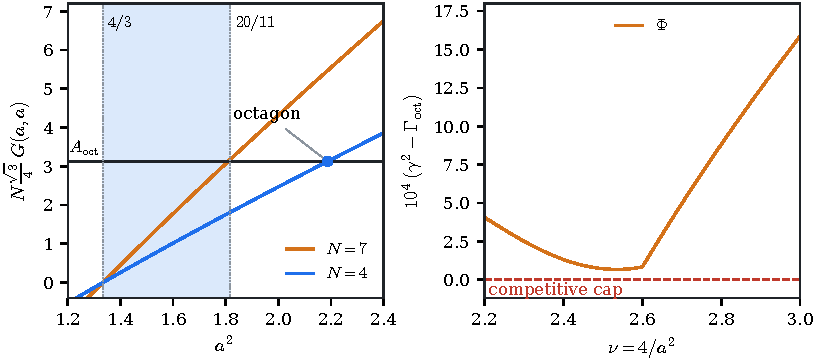
\includegraphics[width=\textwidth]{figures/fig-forward-window.pdf}
\caption{The two sides of the case F contradiction. Left: the cost $N\frac{\sqrt3}4G(a,a)$ of $N$
equal edges against $a^2$, for $N=4$ and $N=7$. Four edges at the octagon's margin cost exactly
$\Aoct$ (dot). Seven edges cost more than $\Aoct$ once $a^2\ge20/11$ (\cref{lem:fwd-threshold}),
and $a^2>4/3$ by \cref{lem:fwd-small}, so the least active margin of a long competitive forward
period lies in the shaded band. Right: on that band, under the bounds of
\cref{lem:fwd-budget,lem:fwd-neighbour,lem:fwd-norms}, the Casimir is at least the smaller of
the two curves $\phi_A,\phi_B$ of \cref{app:fwd-casimir}, which stay above $23/125$, while competitiveness forces $\gamma^2<0.18381$ (dashed). The vertical
scale is $10^{4}(\gamma^2-23/125)$.}\label{fig:forward}
\end{figure}
